% -----------------------------------------------------------------------------
\section{Examples}\label{sec:examples}
% -----------------------------------------------------------------------------

This section contains prototypical examples, including use of all
current glyphs to attempt to ensure that their use is clear.

\begin{figure}[h!]

\includegraphics[scale=0.5]{figures/apdx-examples/apdx-exa1.pdf}
\caption{DNA sequence for a functional unit in which the pTet promoter and an anonymous 5'UTR regulate expression of a coding sequence for GFP, ended by a terminator.}
\label{f:apdx:exa1}
\end{figure}

\begin{figure}[h!]

\includegraphics[scale=0.5]{figures/apdx-examples/apdx-exa2.pdf}
\caption{The same functional unit as in \ref{f:apdx:exa1}, with additional assembly-focused information: there is a 5' overhang before the promoter, a 3' overhand after the terminator, and an assembly scar between the promoter and the 5'UTR left over from a prior step of assembly.}
\label{f:apdx:exa2}
\end{figure}

\begin{figure}[h!]
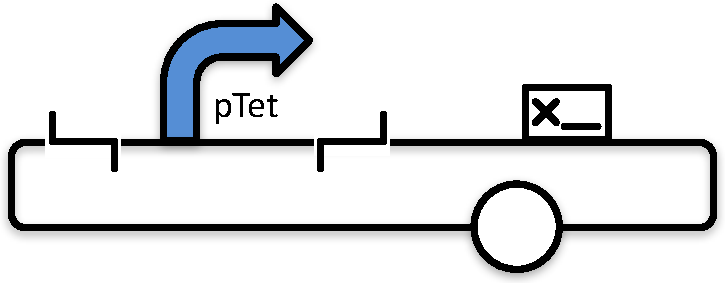
\includegraphics[scale=0.5]{figures/apdx-examples/apdx-exa3.pdf}
\caption{Promoter pTet stored in a circular plasmid. The promoter is prepared for being cut out of the plasmid: it is preceded by a 5' sticky end restriction site and followed by a 3' stick end restriction site.  In addition, the plasmid has been bar-coded with a signature and has its origin of replication marked.}
\label{f:apdx:exa3}
\end{figure}

\begin{figure}[h!]
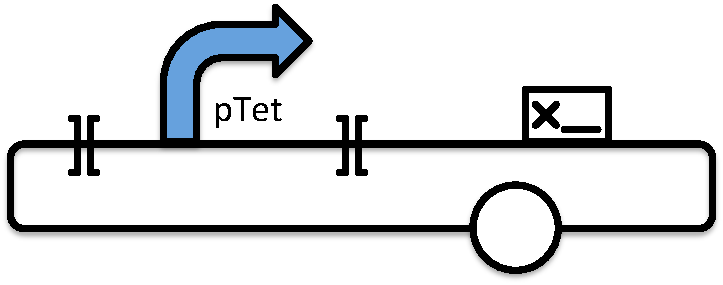
\includegraphics[scale=0.5]{figures/apdx-examples/apdx-exa4.pdf}
\caption{Promoter stored in a plasmid as in \ref{f:apdx:exa3}, except that the restriction sites before and after the promoter are blunt-end.}
\label{f:apdx:exa4}
\end{figure}

\begin{figure}[h!]
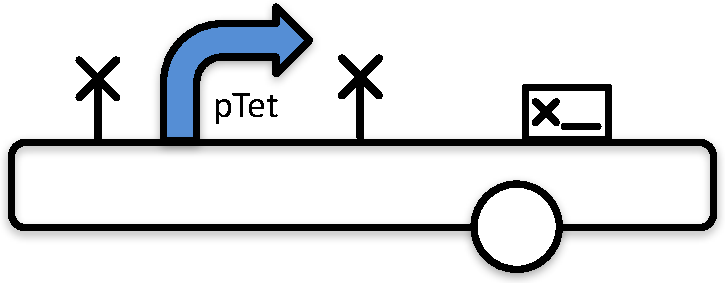
\includegraphics[scale=0.5]{figures/apdx-examples/apdx-exa5.pdf}
\caption{Promoter stored in a plasmid as in \ref{f:apdx:exa3}, except that the cut structure of the restriction sites before and after the promoter is not specified.}
\label{f:apdx:exa5}
\end{figure}

\begin{figure}[h!]
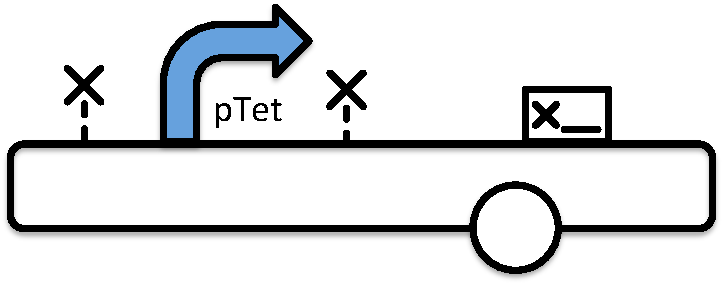
\includegraphics[scale=0.5]{figures/apdx-examples/apdx-exa6.pdf}
\caption{Promoter stored in a plasmid as in \ref{f:apdx:exa3}, except that the promoter is described as being flanked by nuclease sites rather than restriction sites.}
\label{f:apdx:exa6}
\end{figure}

\begin{figure}[h!]
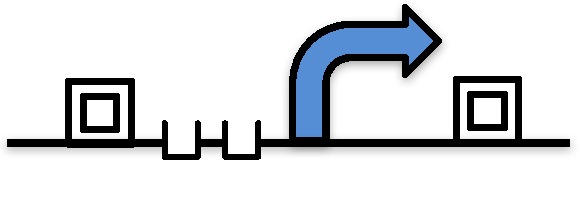
\includegraphics[scale=0.5]{figures/apdx-examples/apdx-exa7.pdf}
\caption{Detailed design of a promoter, in which the transcription start site is preceded by two operator sites where regulators bind, and the whole is flanked by insulators.}
\label{f:apdx:exa7}
\end{figure}

\begin{figure}[h!]
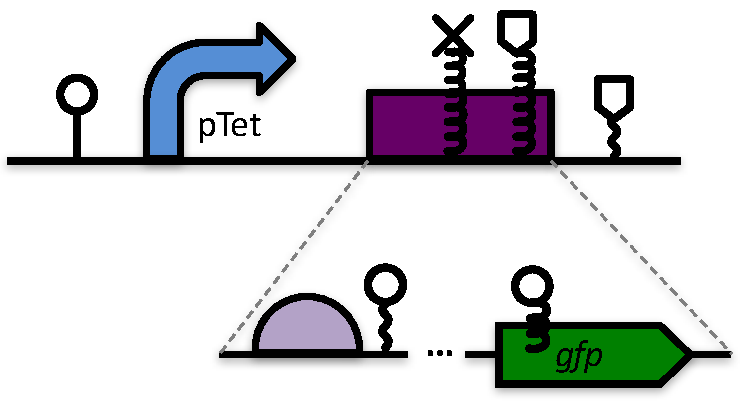
\includegraphics[scale=0.5]{figures/apdx-examples/apdx-exa8.pdf}
\caption{Promoter regulating the production of a user-defined composite sequence that includes RNA and protein stability elements at its 3' end, as well as an internal site for protease cleavage, as well as the expansion of the composite to show it contains a 5'UTR. coding sequence, and other omitted details}
\label{f:apdx:exa8}
\end{figure}

\begin{figure}[h!]
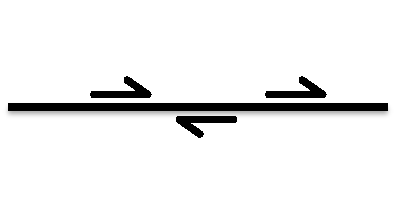
\includegraphics[scale=0.5]{figures/apdx-examples/apdx-exa9.pdf}
\caption{DNA sequence with three primer binding sites.}
\label{f:apdx:exa9}
\end{figure}

\begin{figure}[h!]
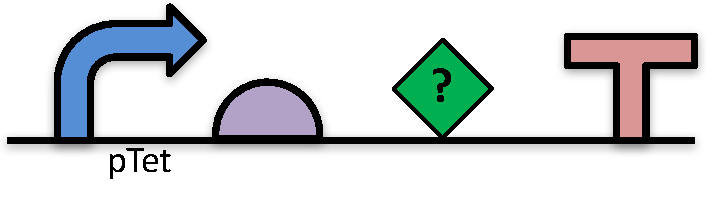
\includegraphics[scale=0.5]{figures/apdx-examples/apdx-exa10.pdf}
\caption{The same functional unit as in \ref{f:apdx:exa1}, except that information about the CDS is missing, leaving it to be fall back on the default unspecified glyph.}
\label{f:apdx:exa10}
\end{figure}

\begin{figure}[h!]
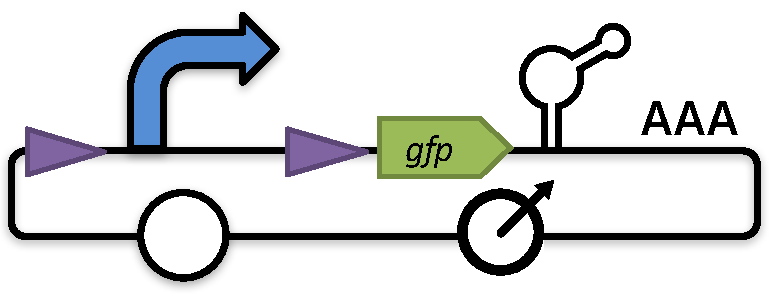
\includegraphics[scale=0.5]{figures/apdx-examples/apdx-exa11.pdf}
\caption{Promoter regulating the expression of GFP, which is also regulated by an aptamer between it and the poly-A tail of the transcript. The promoter can be cut out by a pair of recombinase target sites.  The whole construct is stored in a circular plasmid with an origin of replication and also an origin of transfer.}
\label{f:apdx:exa11}
\end{figure}

% Figure black magic: adjust the size here as needed to get the spacing on the last page of the section correct.
%\begin{figure}[h!]
%\vspace{5in}
%\end{figure}
